\documentclass[12pt]{ICSPoster}

%\usepackage[german]{babel}

\newenvironment{algorithmUmg}{\begin{small}\begin{tabular}{|l|}\hline}{\\ \hline \end{tabular}\end{small}}

\newcommand{\norm}[2]{\|{#1}\|_{#2}}

\graphicspath{{./figures/}}

\title{Applied Mathematics\\[0.2cm]and Computational Science}
% optional subtitle
\subtitle{High Performance Approach to Cardiac\\ Resynchronization Therapy}
\logo{USI-ICS.jpg} % optional logo default is USI-ICS.jpg

\begin{document}
  \maketitle

  \begin{posterbox}[2]
    \begin{headerbox}[
        title=Background: Understanding Cardiac Resynchronization Therapy,
        height=0.23\textheight,
        width=0.47\textwidth]
      \begin{minipage}{\textwidth}\sf
        \textbf{Background}
        \vspace{1mm}
        \begin{compactitem}
          \item Heart failure is a major health problem: $\sim 5$ million affected patients alone in Europe
          \item High direct and indirect treatment costs
        \end{compactitem}
      \end{minipage}

      \vspace{0.5cm}

      \begin{minipage}{0.55\textwidth}\sf
        \textbf{Cardiac Resynchronization Therapy (CRT)}
        \begin{compactitem}
          \item Left bundle branch block: Failure in electrical activation system
          \item Leads to discoordinated contraction and poor pump function
          \item CRT: Implantable pacemaker connected to a pacing electrode
                located in each of the main cardiac chambers
          \item Aim: Reduce total time of activation and improve synchrony
          \item Treatment effective for some patients: Reduces mortality and hospitalization rate
          \item Problem: Other patients show no change at all or even develop cardiac arrhythmia
        \end{compactitem}

        \vspace{0.5cm}

        \textbf{Relevant Questions}
        \begin{compactitem}
          \item How to predict the success/failure of CRT using practical techniques like electrocardiograms (ECGs)
          \item Identify and separate anatomical and electrophysiological changes due to CRT
          \item Final Goal: Provide practical guidelines about optimal site, tailored device programming
                and easy-to-use follow-up criteria
        \end{compactitem}

      \end{minipage}
      \begin{minipage}{0.25\textwidth}\sf
        \vspace{0.5cm}
        \hspace{1cm}
        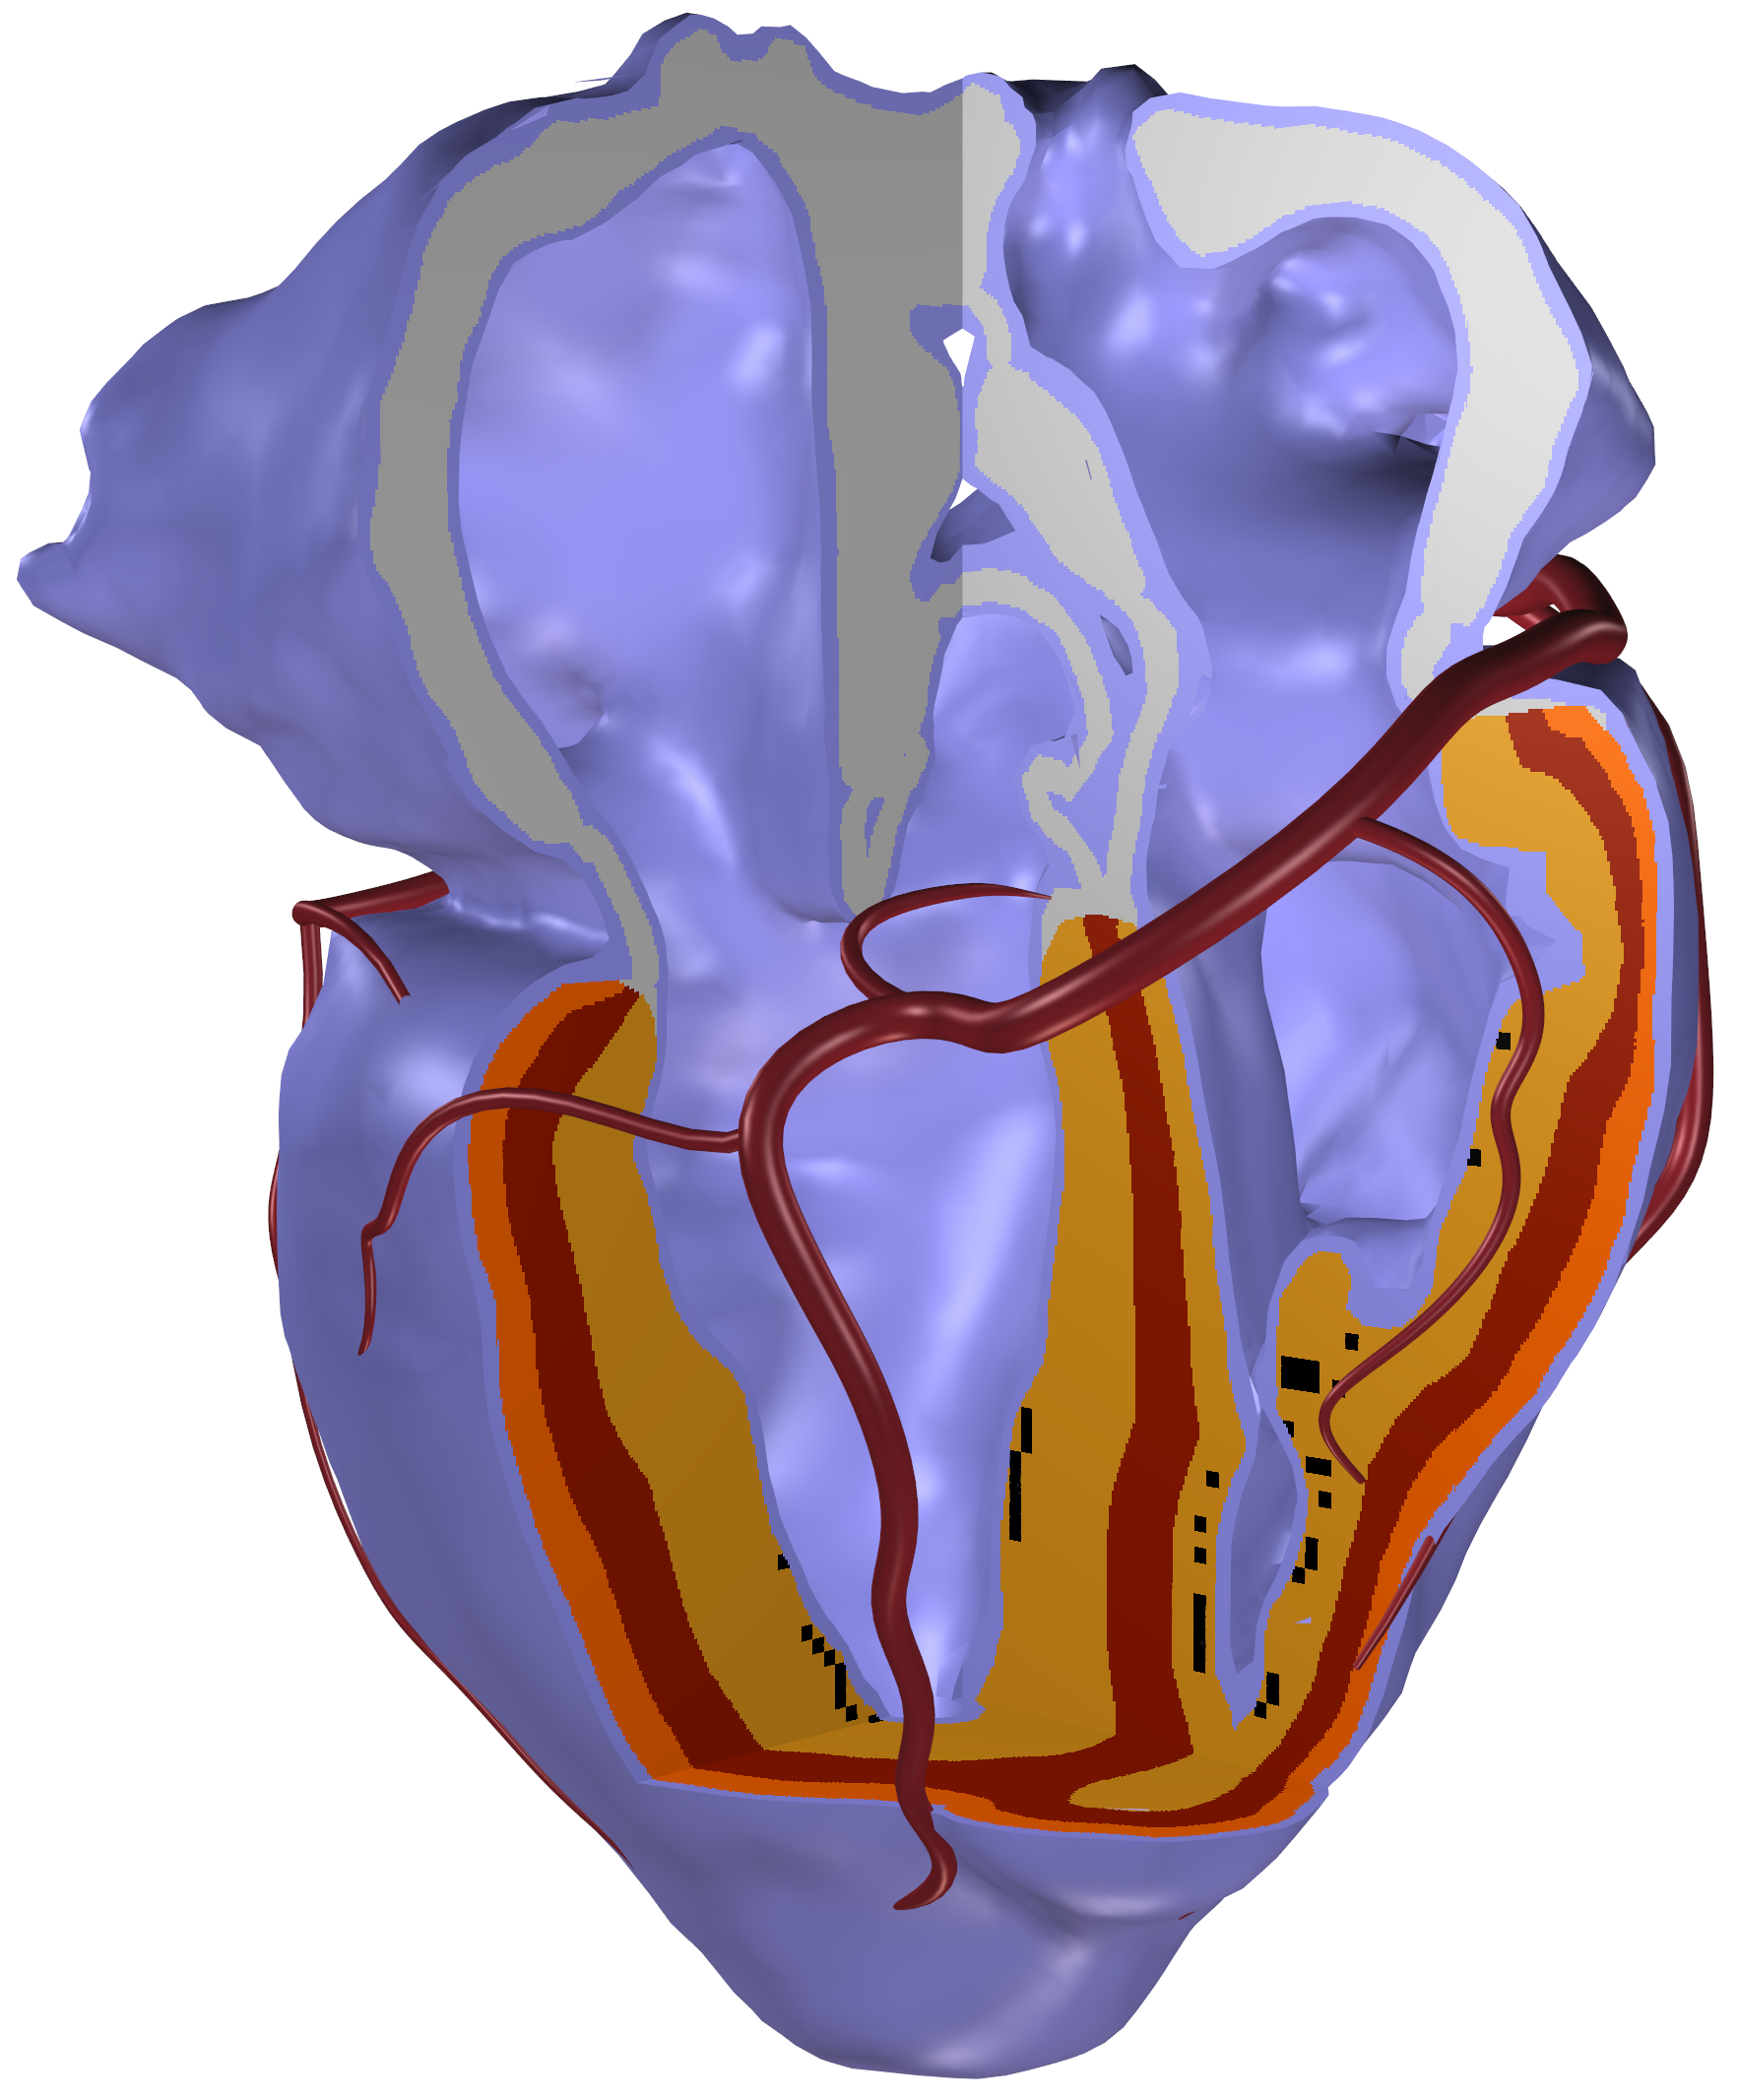
\includegraphics[height=1.8\textwidth]{anatomy.png}
        \begin{flushright}
        {\tiny \copyright Mark Potse, University Maastricht}
        \end  {flushright}
      \end{minipage}

    \end{headerbox}
    \vfill
    %---------------------------------------------------------------------------

    \begin{headerbox}[
        title=Modeling Aspects,
        width=0.47\textwidth,
        height=0.215\textheight]
      \begin{minipage}{\textwidth}\sf
        \textbf{Bidomain Equation}
        \begin{center}
          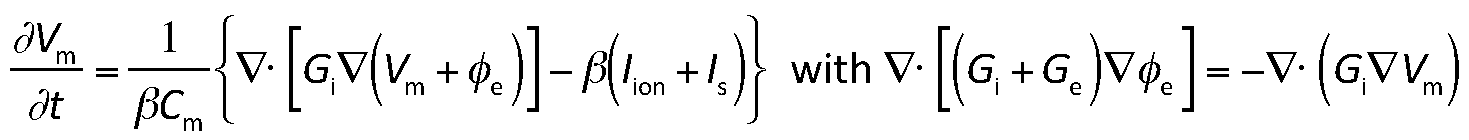
\includegraphics[scale=0.65]{Bidomain}
        \end{center}
        \vspace{-0.25cm}
        \begin{compactitem}
          \item Reaction-diffusion model for the transmembrane potential
                $\text{\sf\textit V}_\text{\!m} = \phi_\text{i} - \phi_\text{e}$
                with intracellular/extra-\\cellular potentials $\mathsf \phi_\text{i}$ and
                $\mathsf \phi_\text{e}$
          \item Ionic part $\text{\sf\textit I}_\text{ion} =
                \text{\sf\textit I}_\text{ion}(\text{\sf\textit V}_\text{\!m},\text{\sf\textit t})$ of
                the transmembrane current density computed by a membrane model
        \end{compactitem}

        \vspace{0.25cm}
      \end{minipage}

      \begin{minipage}{0.35\textwidth}\sf
        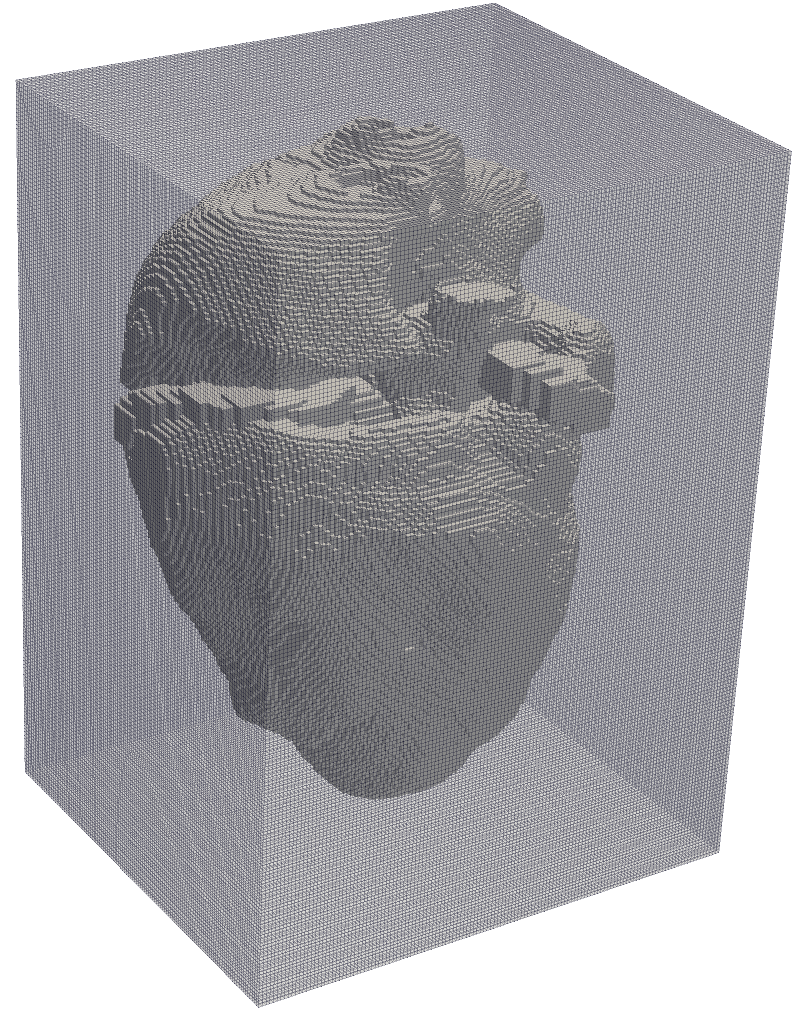
\includegraphics[width=\textwidth]{pic_heart_box.png}
      \end{minipage}
      \begin{minipage}{0.50\textwidth}\sf
        \textbf{Monodomain Equation}
        \begin{center}
          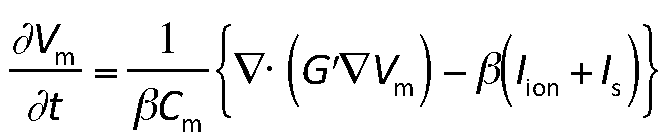
\includegraphics[scale=0.55]{Monodomain}
        \end  {center}
        \vspace{-0.25cm}
        \begin{compactitem}
          \item Derived from bidomain model assuming scalar relation between intra- and extracellular
                conductivities and the ``bulk conductivity tensor'' $\text{\textsf{\textit{G}}}$'
        \end{compactitem}

        \vspace{0.5cm}

        \textbf{Discretization}
        \vspace{1mm}
        \begin{compactitem}
          \item Voxel geometry, \textit{O}(mm) resolution
          \item Second-order finite difference approximation of anisotropic Laplacian
          \item Explicit or implicit time integration
        \end{compactitem}

      \end{minipage}
    \end{headerbox}
  \end{posterbox}

  %%%%%%%%%%%%%%%%%%%%%%%%%%%%%%%%%%%%%%%%%%%%%%%%%%%%%%%%%%%%%%%%%%%%%%%%%%%%%%
  %%%%%%%%%%%%%%%%%%%%%%%%%%%%%%%%%%%%%%%%%%%%%%%%%%%%%%%%%%%%%%%%%%%%%%%%%%%%%%
  \begin{posterbox}[2]
    \begin{headerbox}[
        title=End-to-End Workflow,
        height=0.25\textheight,
        width=0.47\textwidth]
      \begin{minipage}{\textwidth}\sf
        \textbf{Project Partners}
        \begin{compactitem}
          \item Prof.~A.~Aurrichio, Fondazione Cardiocentro Ticino
          \item Prof.~F.~Prinzen, Dr.~M.~Potse, Maastricht University
          \item Prof.~R.~Krause, Dr.~T.~Dickopf, D.~Krause, J.~Steiner, L.~Blondel,\\ Institute of Computational Science, USI
        \end{compactitem}
        \vspace{0.5cm}

        \textbf{Workflow Diagram}

        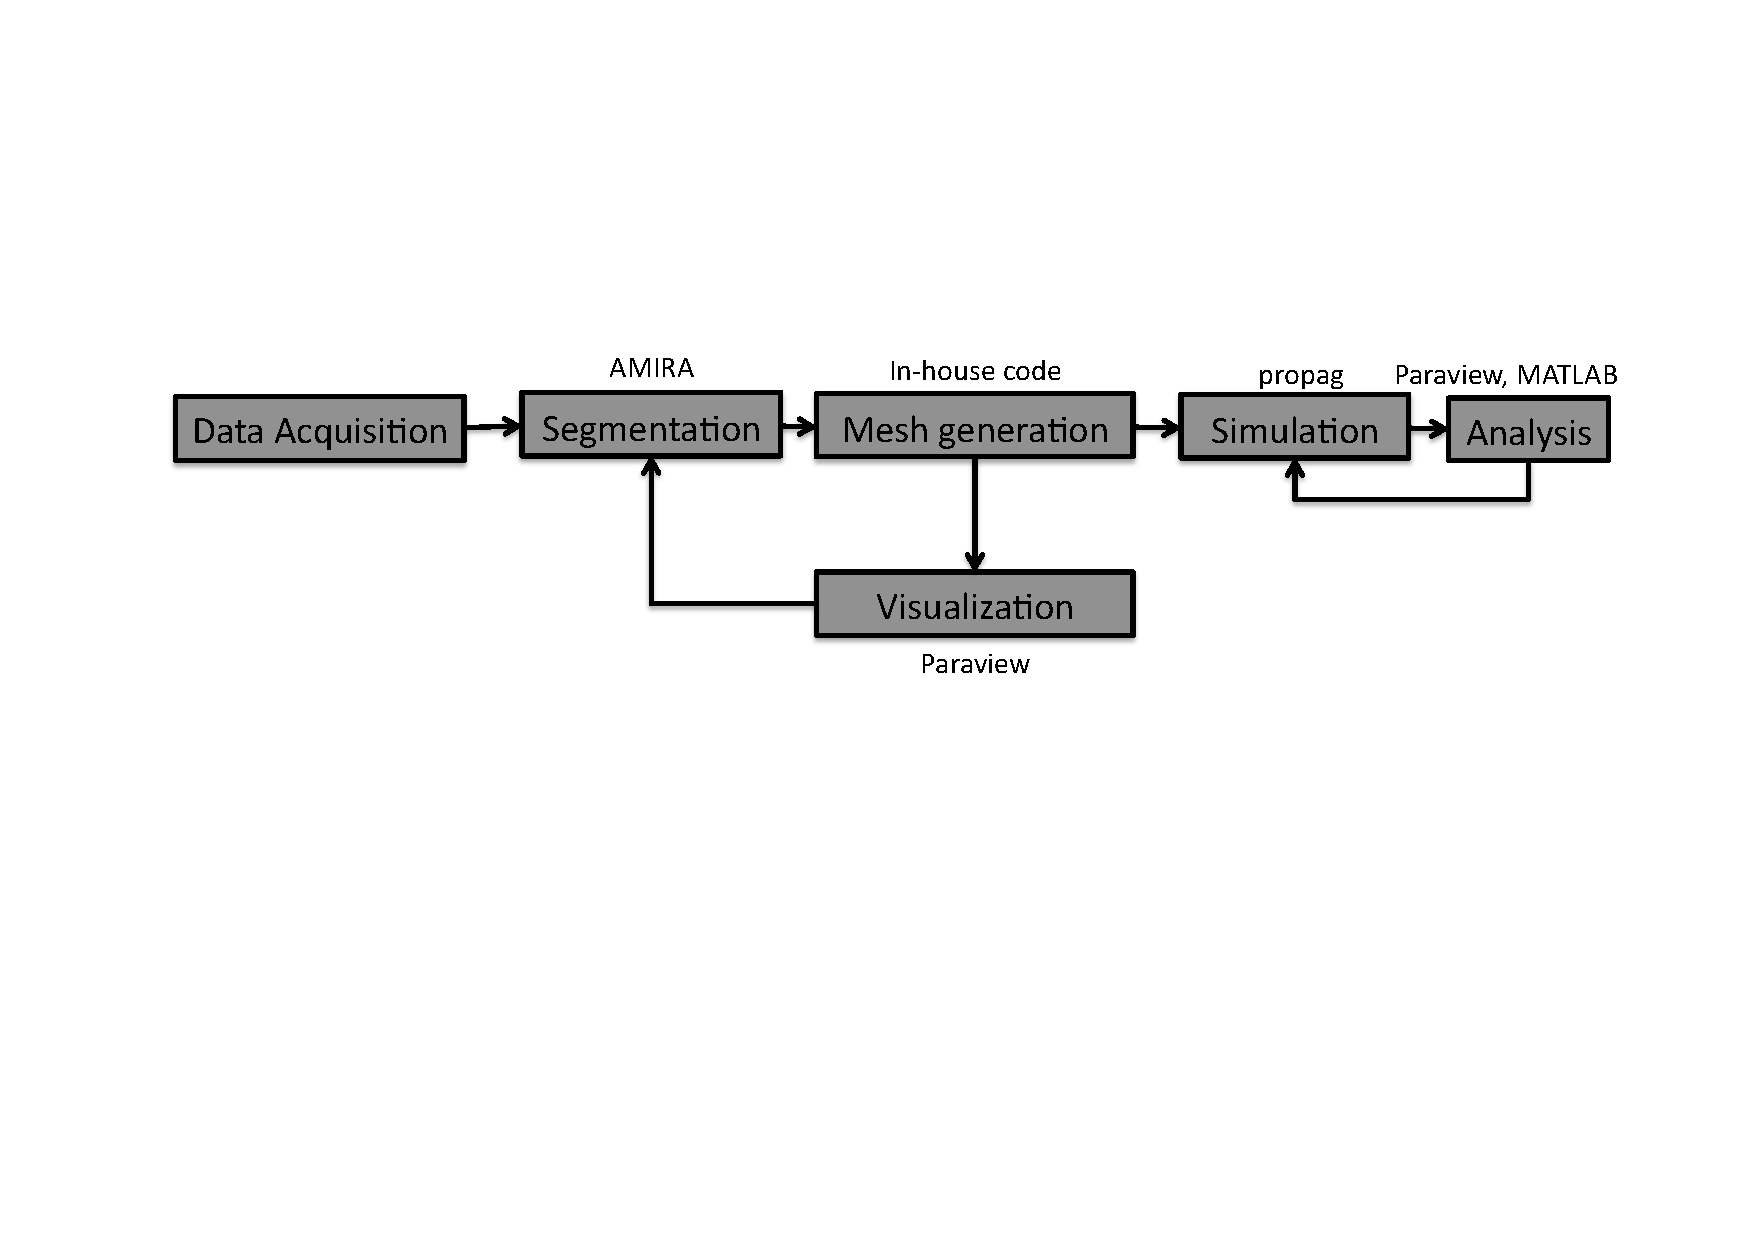
\includegraphics[width=\textwidth]{Workflow}
      \end{minipage}

      \begin{minipage}{0.40\textwidth}\sf
        \textbf{Description}
        \begin{compactitem}
          \item Data Acquisition by clinical partners: MRI, CT images, ECG
          \item Segmentation: Create high-quality surface representation from medical images,
                requires manual detection of anatomical structure
          \item Mesh generation: Create voxel approximation based on surface data
          \item Visualization: Required for steering of process and quality assurance, challenging
                due to high data volume
        \end{compactitem}
      \end{minipage}
      \begin{minipage}{0.40\textwidth}\sf
        \hspace{2cm}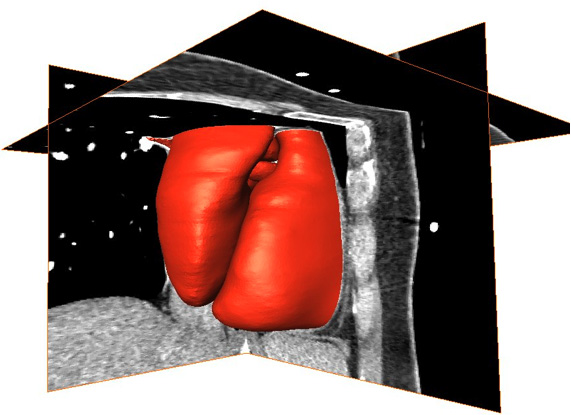
\includegraphics[width=\textwidth]{AMIRA}
      \end{minipage}
    \end{headerbox}
    %----------------------------------------------------------------------------

    \begin{headerbox}[
        title=A Case for High Performance Computing,
        height=0.25\textheight,
        width=0.47\textwidth]
      \textbf{Challenge}
      \begin{compactitem}
        \item Simulate large amount of patient-specific geometries with various
              parameters: requires fast execution\ of forward model
        \item Patient-specific geometries require high number of voxels: $\sim 80$M nodes
        \item Need to scale-out code on high number of cores
        \item Utilize massively parallel supercomputers such as \textit{Rosa} at CSCS
              (Swiss National Supercomputing Centre\\ in Manno) with 22k cores
      \end{compactitem}

      \vspace{0.5cm}

      \textbf{Achievements}
      \begin{compactitem}
        \item We have scaled-out our production code \textit{propag} on up to 16k cores on \textit{Rosa}
              allowing us to reduce the compute time by orders of magnitudes
        \item Best scaling is achieved by combining two parallel programming models:
              MPI between compute nodes and OpenMP inside nodes
      \end{compactitem}

      \vspace{0.5cm}

      \begin{minipage}{0.5\textwidth}\sf
        \hspace{1cm}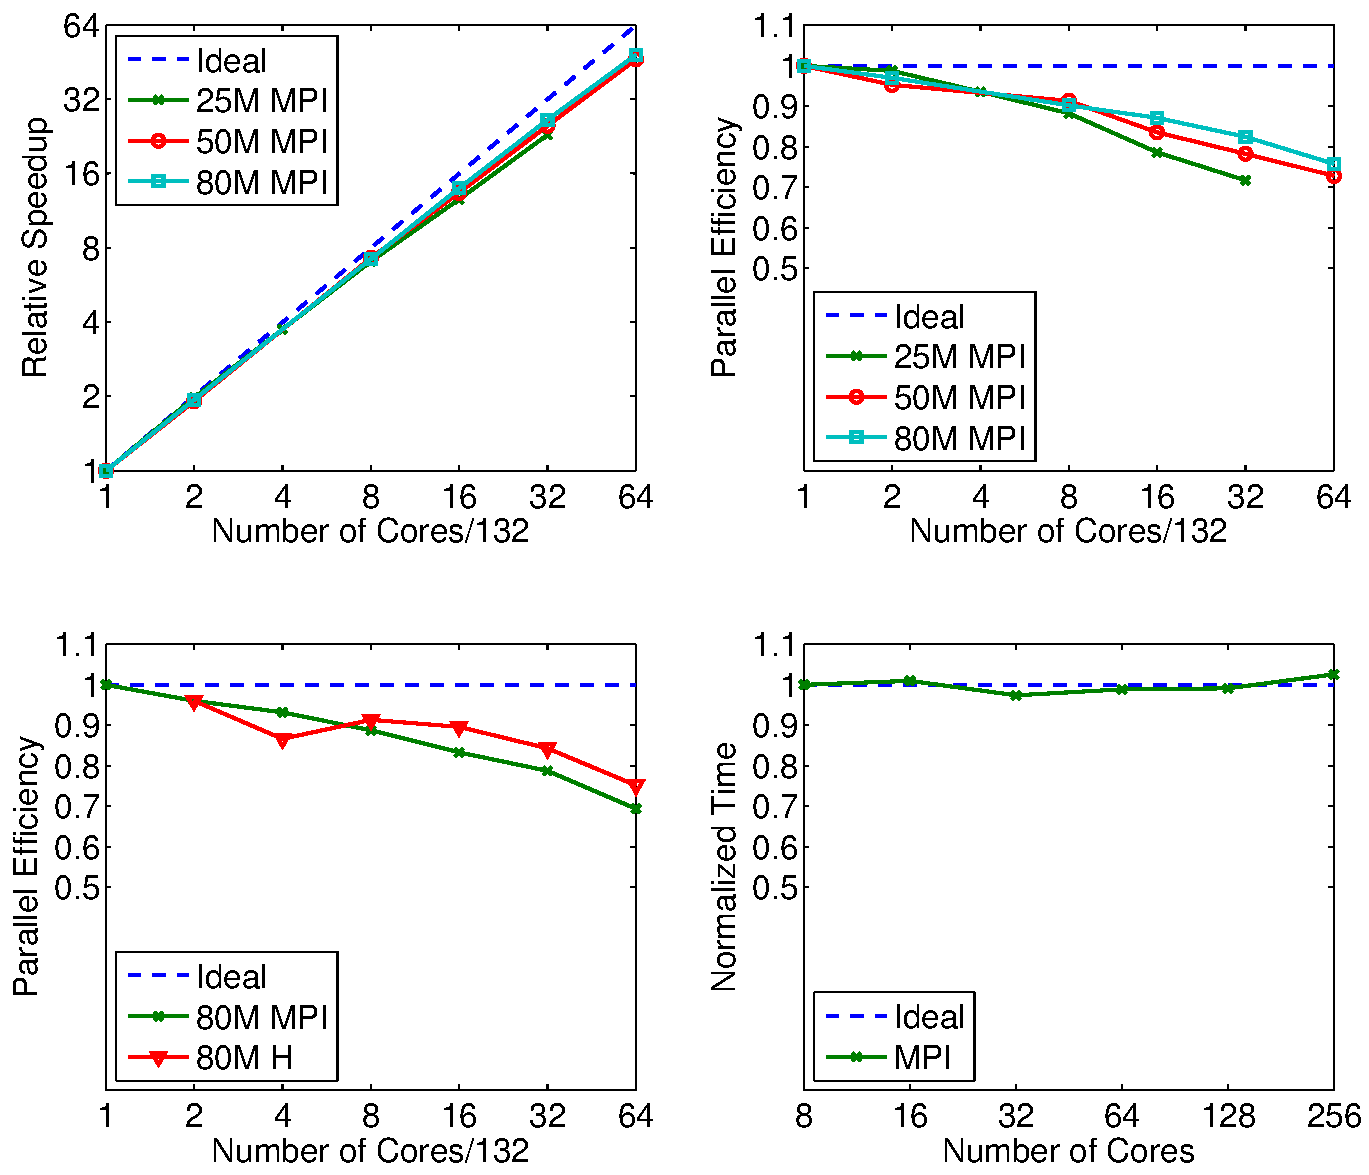
\includegraphics[width=0.9\textwidth]{Scaling}
      \end{minipage}
      \begin{minipage}{0.5\textwidth}\sf
        \begin{center}
          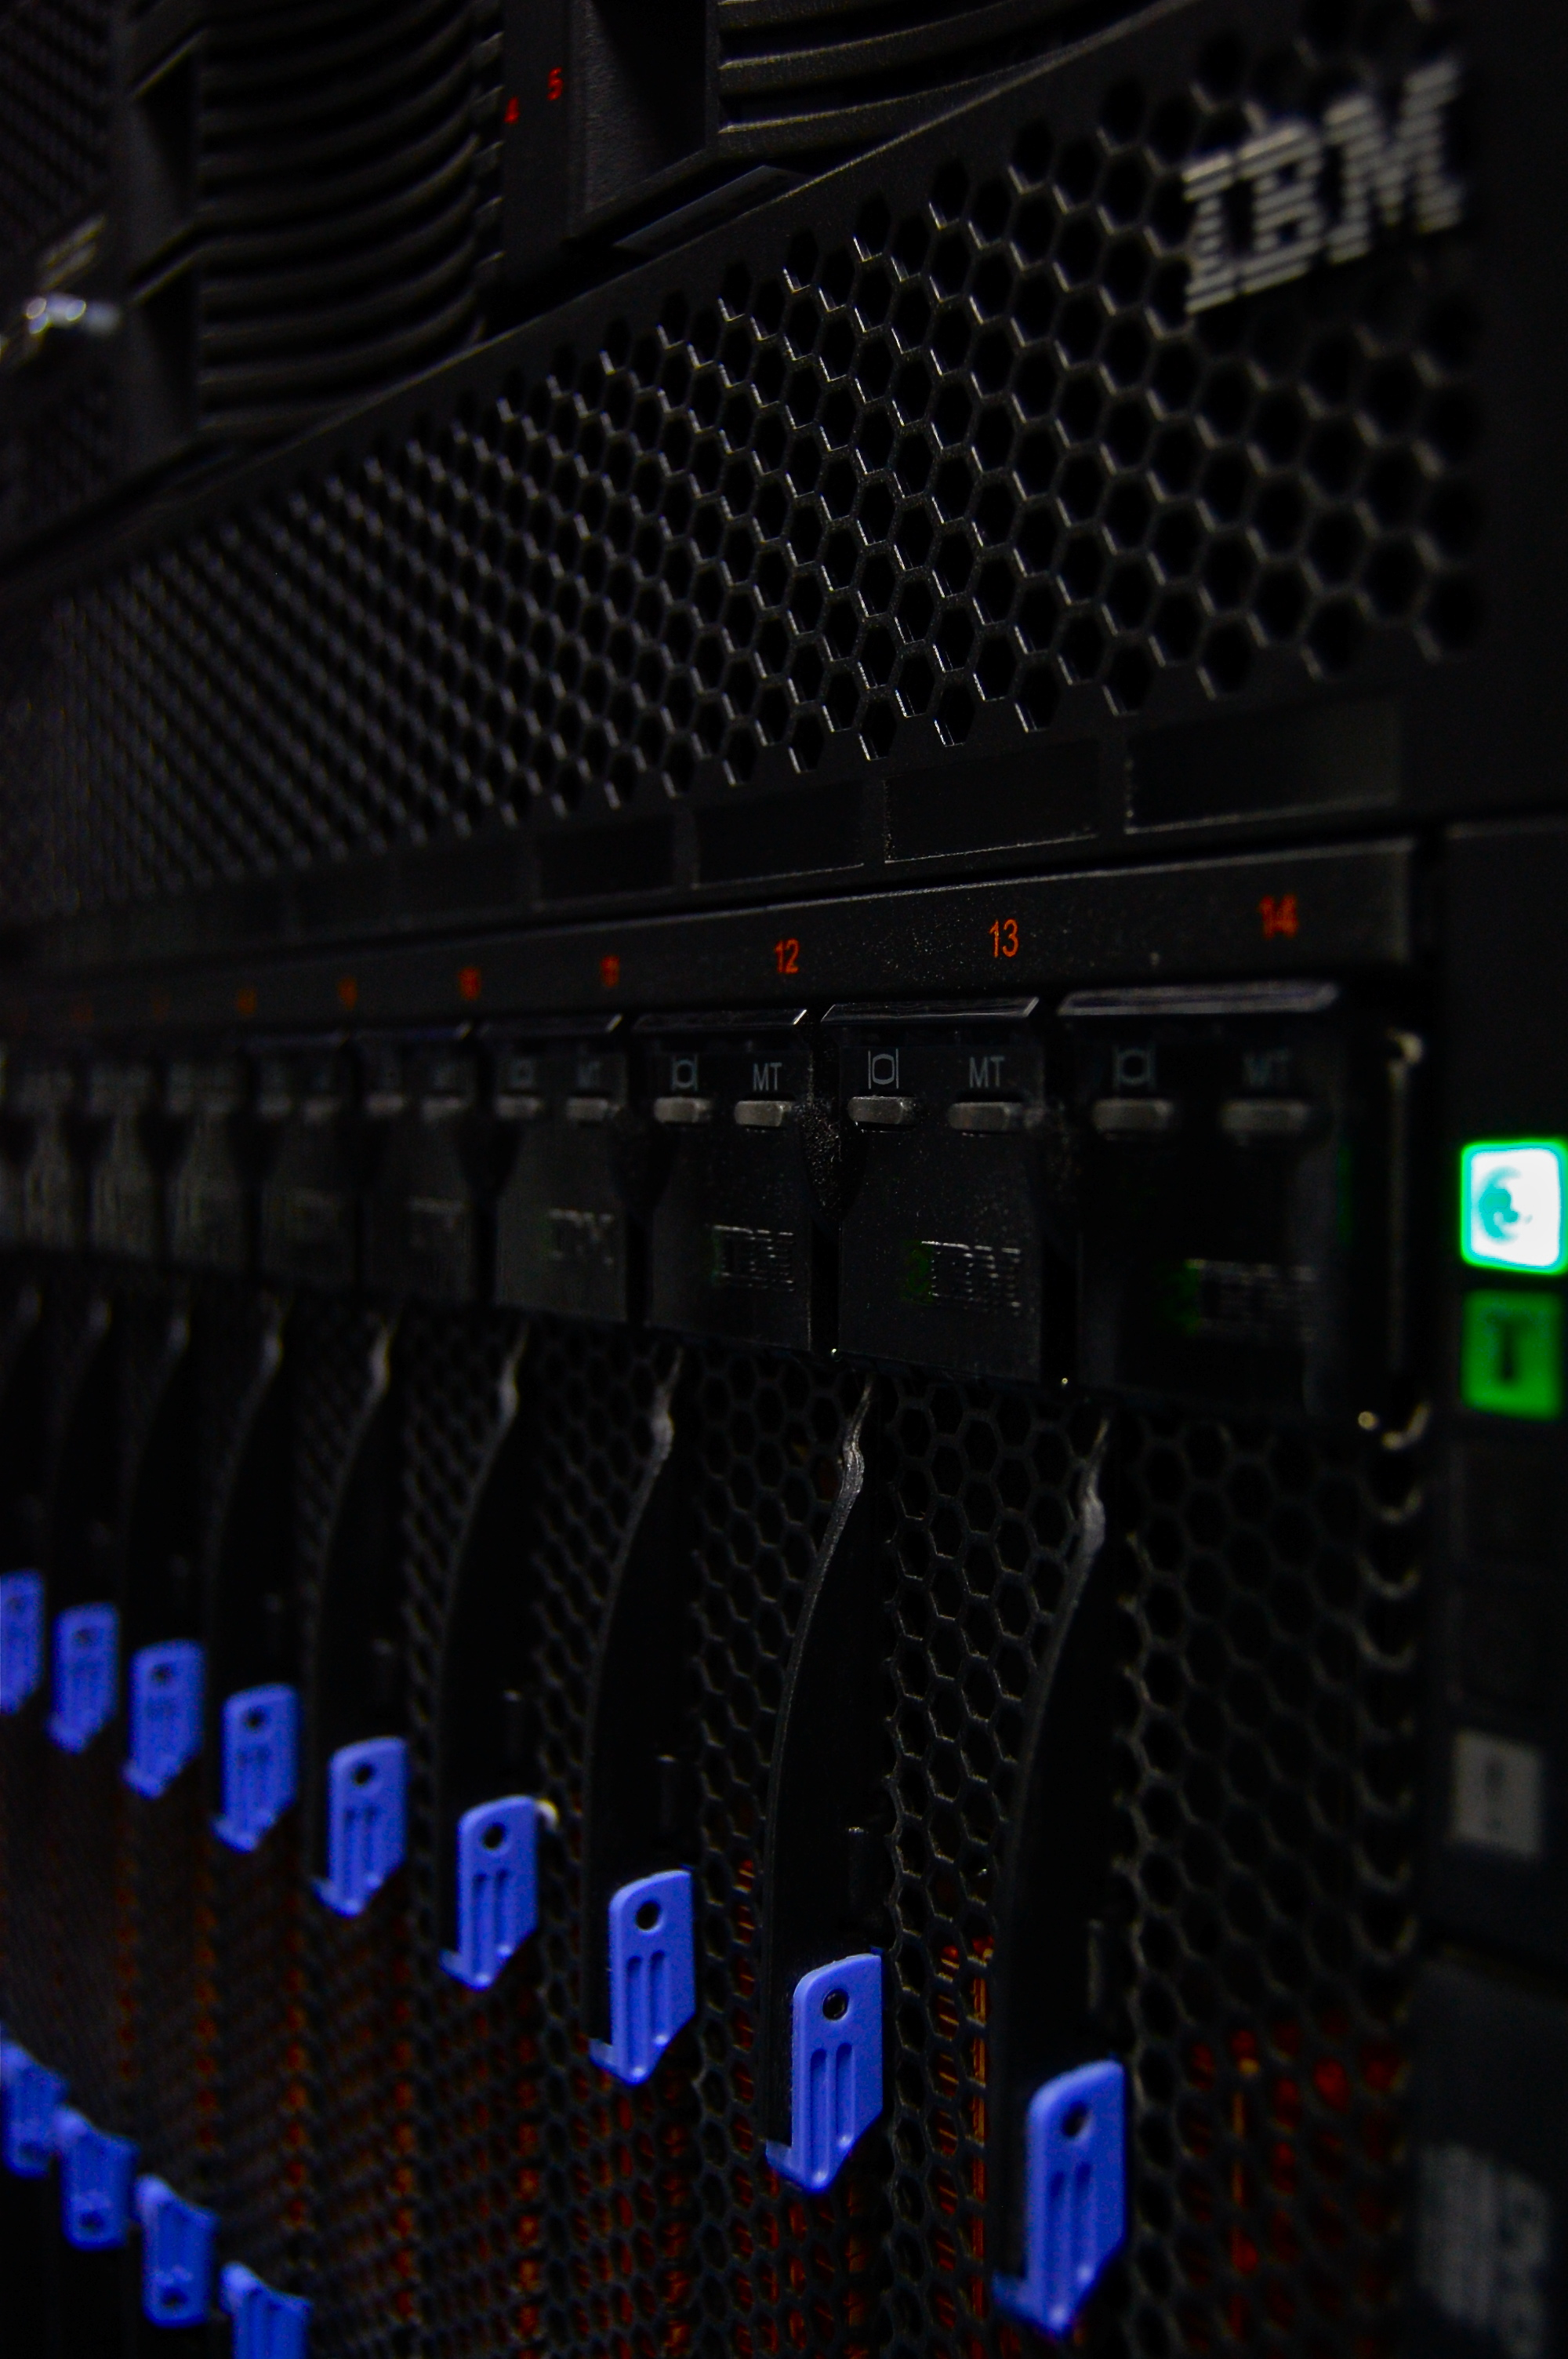
\includegraphics[width=0.5\textwidth]{Cub}
        \end{center}
      \end{minipage}
    \end{headerbox}
  \end{posterbox}

  %%%%%%%%%%%%%%%%%%%%%%%%%%%%%%%%%%%%%%%%%%%%%%%%%%%%%%%%%%%%%%%%%%%%%%%%%%%%%%
  %%%%%%%%%%%%%%%%%%%%%%%%%%%%%%%%%%%%%%%%%%%%%%%%%%%%%%%%%%%%%%%%%%%%%%%%%%%%%%
  \begin{posterbox}
    \begin{headerbox}[
        title=Simulation of a Heartbeat,
        height=0.19\textheight]
      \begin{minipage}{0.19\textwidth}\sf
        \textbf{Description}
        \begin{compactitem}
          \item Monodomain simulation of a full heartbeat
          \item Stimulation current applied at end of Purkinje fibers
          \item Performed on 132 cores of \textit{Rosa} with $\sim 40$ min wallclock time
          \item The visualization shows the steep rise of the transmembrane potential
                and the smooth decay
        \end{compactitem}

        \vspace{0.5cm}

        \textbf{Visualization}
        \begin{compactitem}
          \item Visualization is an essential tool for analysis of simulation data but can
                be a challenge in itself
          \item Visualization (performed by Jean Favre from CSCS) required four visualization nodes
                to allow for handling the massive data volume produced by the time-dependent simulation
        \end{compactitem}
      \end{minipage}
      \begin{minipage}{0.79\textwidth}\sf
        \begin{center}
          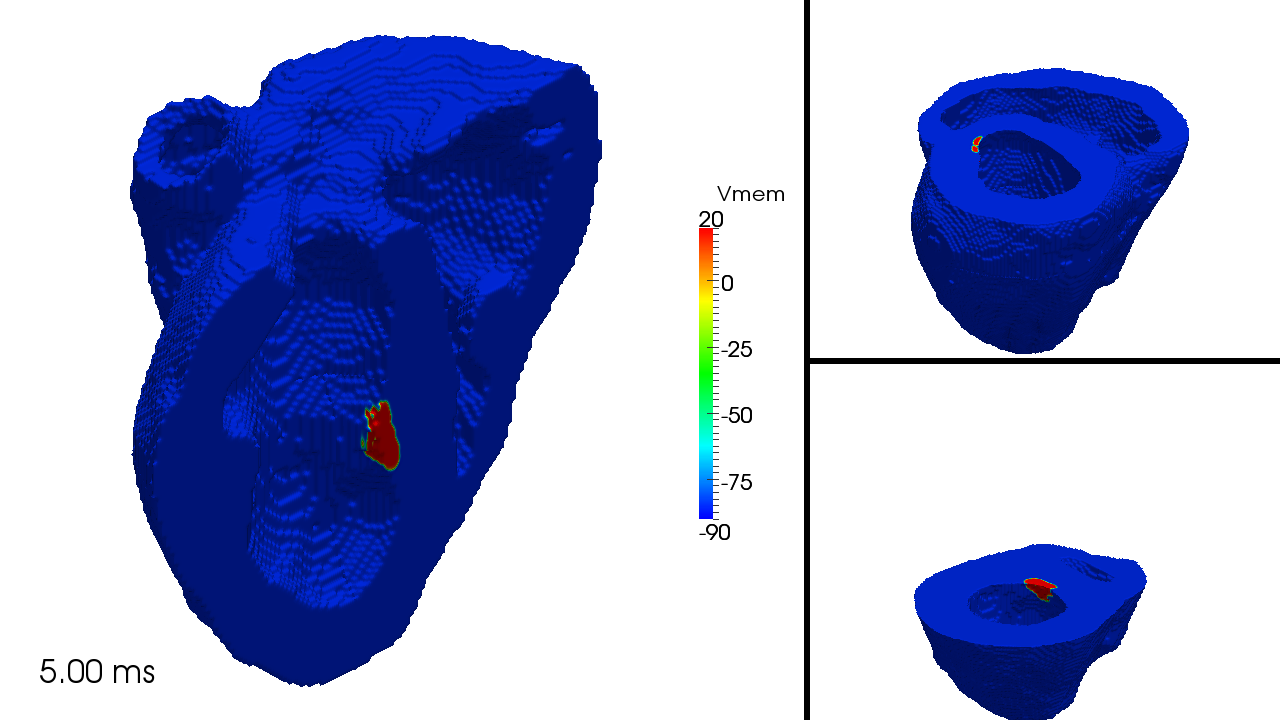
\includegraphics[width=0.3\textwidth]{heart1}
          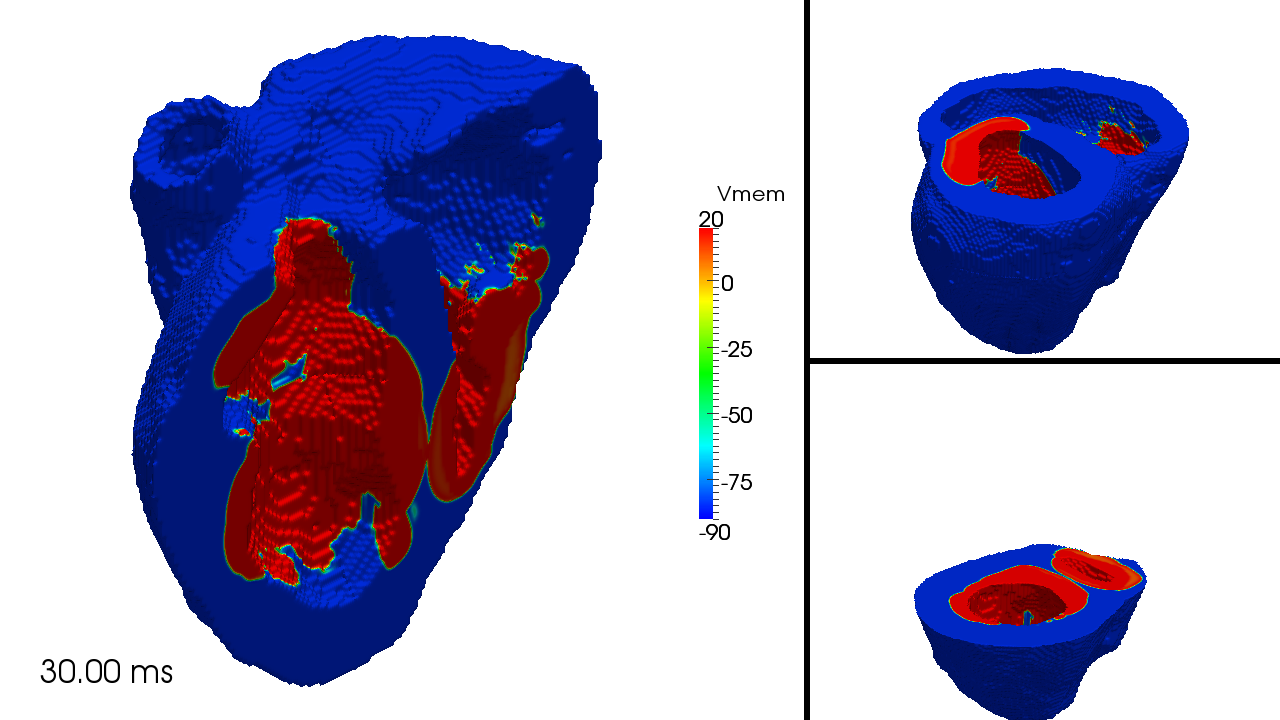
\includegraphics[width=0.3\textwidth]{heart2}
          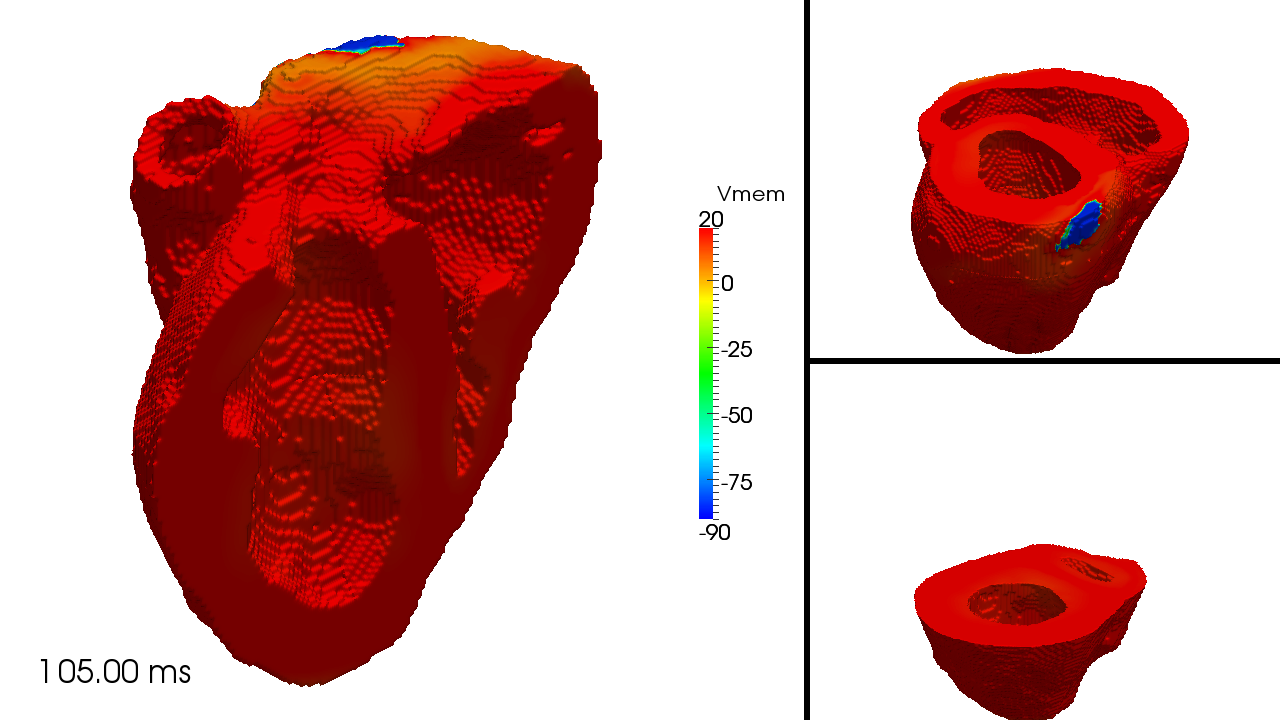
\includegraphics[width=0.3\textwidth]{heart3}
        \end{center}
        \begin{center}
          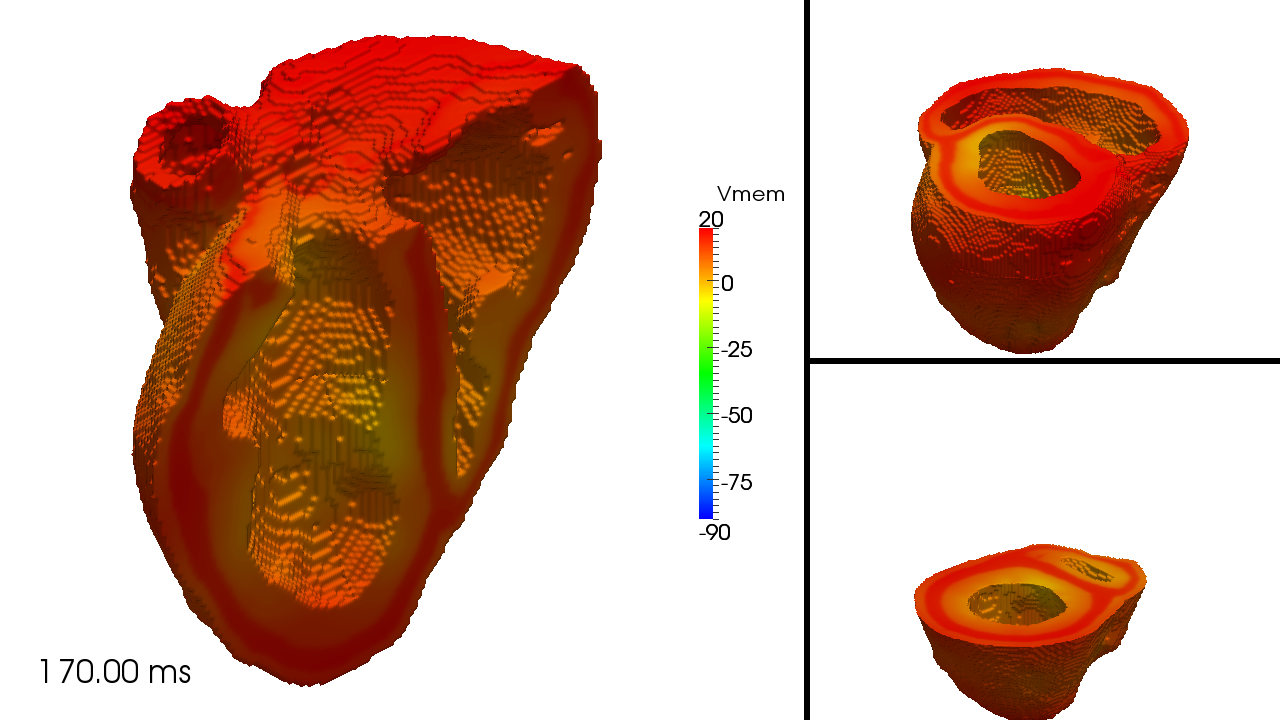
\includegraphics[width=0.3\textwidth]{heart4}
          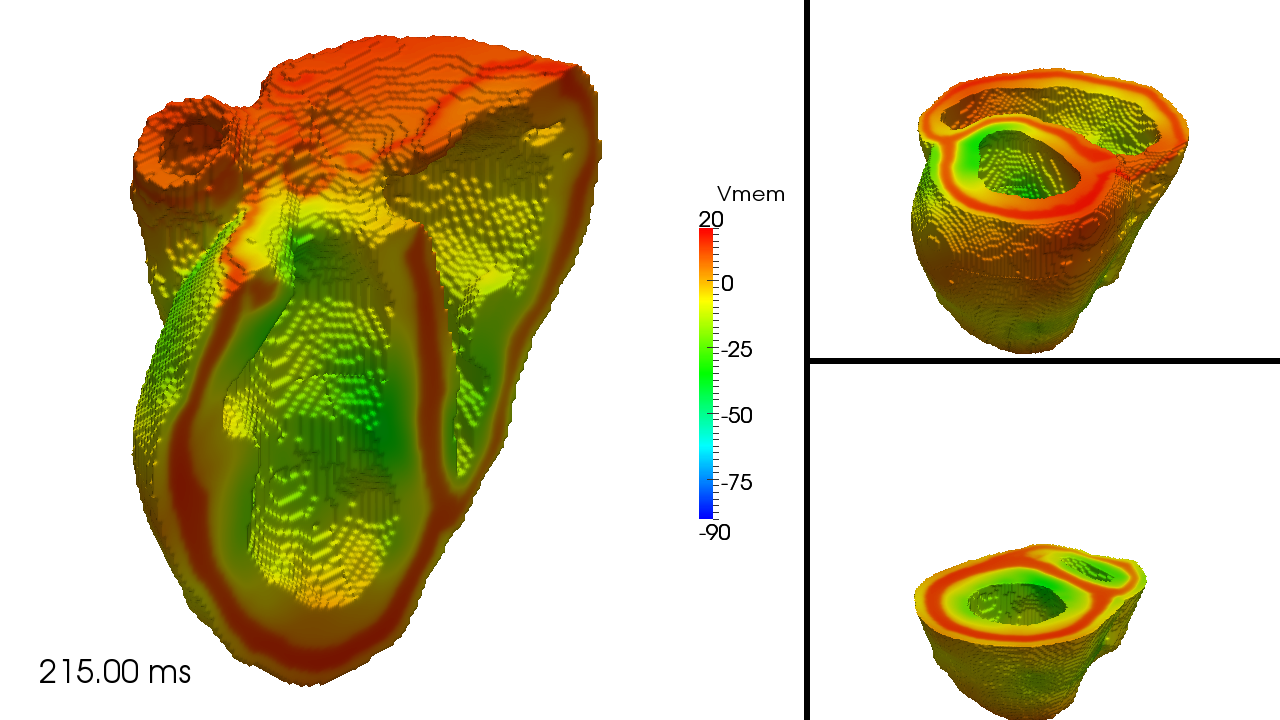
\includegraphics[width=0.3\textwidth]{heart5}
          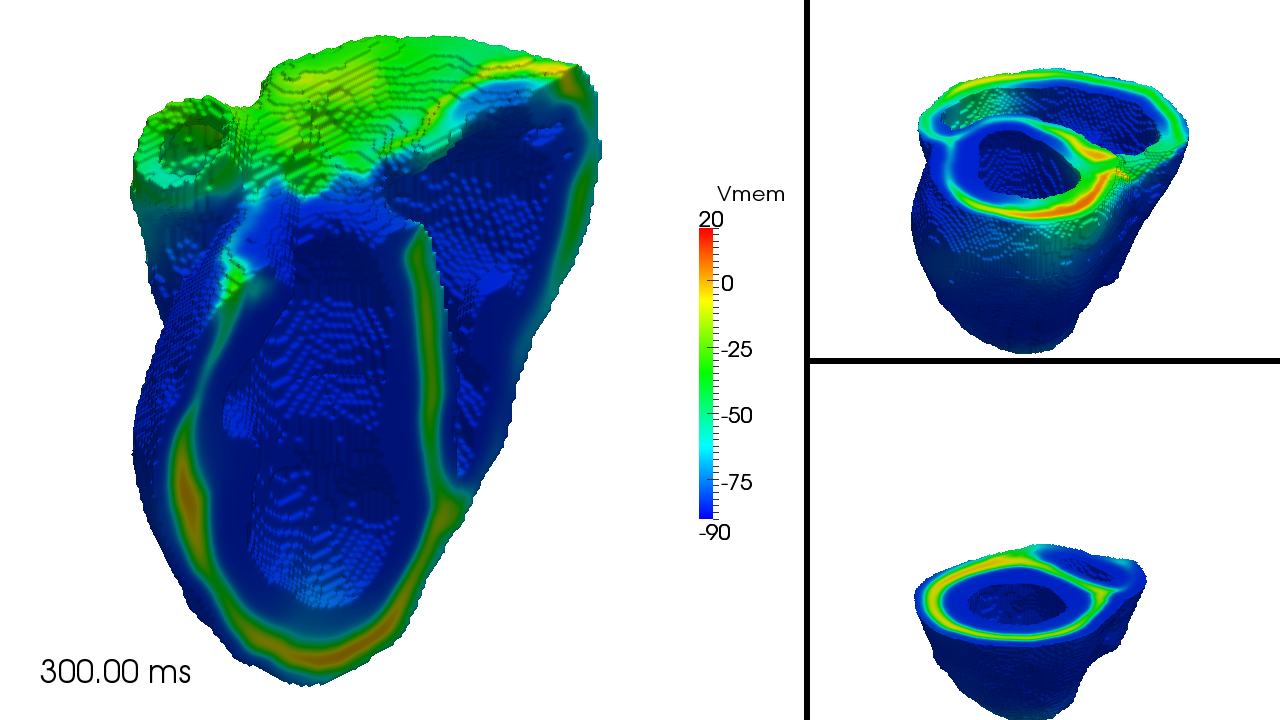
\includegraphics[width=0.3\textwidth]{heart6}
        \end{center}
      \end{minipage}
      \end{headerbox}
  \end{posterbox}

\end{document}
